\documentclass[11pt,a4paper]{scrreprt}

\usepackage[utf8]{inputenc}
\usepackage[italian]{babel}

\usepackage{amsmath}
\usepackage{graphicx}
\usepackage{tabularx}

\usepackage{parskip}

\usepackage{placeins}

\usepackage{url}
\usepackage{fancyvrb}
\usepackage{fancyref}
\usepackage[hidelinks]{hyperref}

\author{L. De Sano, A. Donizetti}
\title{\textsc{FIC}: Fractal Image Compression}
\date{Luglio 2015}

\begin{document}
\maketitle

\tableofcontents

\chapter{Introduzione}

Con il termine ``Fractal image Compression'' si va ad indicare una famiglia di tecniche di compressione di immagini (o video) basate sulle proprietà matematiche dei frattali. Tali metodi di compressione si rivelano sopra ogni altra cosa adatti a comprimere textures e immagini naturali, o, più in generale, immagini che sono caratterizzate da un elevato livello di \emph{self-similarity} (ovvero aventi delle parti che, al netto di rotazioni e ingrandimenti/riduzioni, somigliano ad altre parti dell'immagine).

La compressione di immagini tramite frattali (così come altre, più diffuse, ad esempio \textit{JPEG}) appartiene a quel gruppo di tecniche di compressione \emph{lossy}, ovvero in cui la compressione dell'immagine avviene al costo di una perdita di informazione. Tuttavia, a differenza di quanto accade quando si utilizza uno dei metodi di compressione basati sui pixel (come \textit{JPEG}, \textit{GIF} o \textit{MPEG}), nella compressione frattale nessuna parte dell'immagine viene effettivamente memorizzata. Ciò che viene memorizzato è invece la \emph{struttura interna} dell'immagine (ad esempio un indice di quali parti, effettuate le dovute trasformazioni, sono simili ad altre parti). 

Poiché nessun pixel dell'immagine originale viene memorizzato, la decompressione parte da un singolo pixel, di colore qualsiasi, e procede alla ricostruzione dell'immagine originale applicando iterativamente una mappa ricavata dalla struttura interna dell'immagine originale.

In questo documento tratteremo delle tecniche di compressione di immagini basate su frattali, iniziando con una panoramica teorica del loro funzionamento, proseguendo con la discussione di alcuni aspetti pratici e presentando una implementazione giocattolo realizzata in MATLAB, e concludendo infine con alcuni test che consentiranno di valutare praticità e \emph{performances} di una libreria di compressione basata su frattali, anche in confronto con altre tecniche di compressione \emph{Lossy} maggiormente utilizzate.

\chapter{Aspetti teorici}

\section{Introduzione ai frattali}

Un frattale è un oggetto geometrico che si ripete nella sua forma, allo stesso modo, su diverse scale. Questo comportamento fa si che ingrandendo una sua qualsiasi componente si ottiene comunque una figura simile all'originale. In linea di massima possiamo dire che se si considera l'insieme $F$ un frattale, $F$ dovrebbe avere le seguenti proprietà:

\begin{itemize}
\item $F$ ha dettagli ad ogni scala d'ingrandimento;
\item $F$ gode di autosimilitudine (a qualunque scala si osservi, presenta sempre gli stessi caratteri globali);
\item la dimensione frattale di $F$ è maggiore della sua dimensione topologica;
\item esiste un algoritmo relativamente semplice per costruire $F$.
\end{itemize}

% dobbiamo definire dimensione frattale e dimensine topologica? qui c'è qual che serve http://www.vanderbilt.edu/AnS/psychology/cogsci/chaos/workshop/Fractals.html

% mettere qualche esempio di frattale di base con la costruzione iterata?

Un esempio di oggetto geometrico secondo i principi di costruzione di un frattale e che rispetta le proprietà elencate è la curva di \textit{Koch}. La costruzione comincia con una linea di lunghezza $1$ chiamata \textit{initiatior}. Da questa linea si rimuove il terzo centrale e lo si sostituisce con due linee della stessa lunghezza della parte rimossa. Questa nuova forma viene chiamata \textit{generator}. La prima parte della costruzione è mostrata in figura \ref{fig:k1}.

\begin{figure}[!ht]
\centering
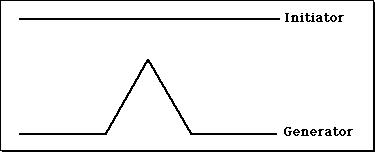
\includegraphics[scale=0.55]{images/koch1.png}
\caption{Initiator e generator per la curca di Koch}
\label{fig:k1}
\end{figure}

La regola può essere nuovamente applicata su ogni linea, così da andare a sostituirla ogni volta come fanno nel passaggio da \textit{initiator} a \textit{generator}. Il secondo livello è visibile in figura \ref{fig:k2}.

\begin{figure}[!ht]
\centering
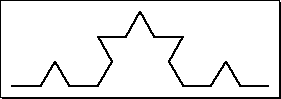
\includegraphics[scale=0.55]{images/koch2.png}
\caption{Livello 2 per la curca di Koch}
\label{fig:k2}
\end{figure}

\FloatBarrier

Una volta che la procedura è avviata può proseguire a piacimento. Il terzo e il quarto livello sono visibili nelle figure \ref{fig:k3} e \ref{fig:k4} rispettivamente.

\begin{figure}[!ht]
\centering
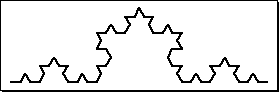
\includegraphics[scale=0.55]{images/koch3.png}
\caption{Livello 3 per la curca di Koch}
\label{fig:k3}
\end{figure}

\begin{figure}[!ht]
\centering
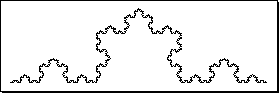
\includegraphics[scale=0.55]{images/koch4.png}
\caption{Livello 4 per la curca di Koch}
\label{fig:k4}
\end{figure}



\section{Iterated Function System}







\end{document}
